\begin{figure*}[th]
\centering
\begin{subfigure}[b]{0.24\textwidth}
\centering
\includegraphics[width=\columnwidth]{data/acc_snli.pdf}
\caption{SNLI (accuracy test)}
\label{fig:cue_snli}
\end{subfigure}
\hfill
\begin{subfigure}[b]{0.24\textwidth}
\centering
\includegraphics[width=\columnwidth]{data/acc_qnli.pdf}
\caption{QNLI (accuracy test)}
\label{fig:cue_qnli}
\end{subfigure}
\hfill
\begin{subfigure}[b]{0.24\textwidth}
\centering
\includegraphics[width=\columnwidth]{data/acc_mnli.pdf}
\caption{MNLI (accuracy test)}
\label{fig:cue_mnli}
\end{subfigure}
\hfill
\begin{subfigure}[b]{0.24\textwidth}
\centering
\includegraphics[width=\columnwidth]{data/acc_roc.pdf}
\caption{ROC (accuracy test)}
\label{fig:cue_mnli}
\end{subfigure}
\hfill
\newpage
\begin{subfigure}[b]{0.24\textwidth}
\centering
\includegraphics[width=\columnwidth]{data/acc_copa.pdf}
\caption{COPA (accuracy test)}
\label{fig:cue_copa}
\end{subfigure}
\hfill
\begin{subfigure}[b]{0.24\textwidth}
\centering
\includegraphics[width=\columnwidth]{data/acc_reclor.pdf}
\caption{RECLOR (accuracy test)}
\label{fig:cue_reclor}
\end{subfigure}
\hfill
\begin{subfigure}[b]{0.24\textwidth}
\centering
\includegraphics[width=\columnwidth]{data/acc_arct.pdf}
\caption{ARCT (accuracy test)}
\label{fig:cue_arct}
\end{subfigure}
\hfill
\begin{subfigure}[b]{0.24\textwidth}
\centering
\includegraphics[width=\columnwidth]{data/acc_arct2.pdf}
\caption{ARCT2 (accuracy test)}
\label{fig:cue_arct2}
\end{subfigure}
\newpage
\begin{subfigure}[b]{0.24\textwidth}
\centering
\includegraphics[width=\columnwidth]{data/dist_snli.pdf}
\caption{SNLI (dist test)}
\label{fig:d_cue_snli}
\end{subfigure}
\hfill
\begin{subfigure}[b]{0.24\textwidth}
\centering
\includegraphics[width=\columnwidth]{data/dist_qnli.pdf}
\caption{QNLI (dist test)}
\label{fig:d_cue_qnli}
\end{subfigure}
\hfill
\begin{subfigure}[b]{0.24\textwidth}
\centering
\includegraphics[width=\columnwidth]{data/dist_mnli.pdf}
\caption{MNLI (dist test)}
\label{fig:d_cue_mnli}
\end{subfigure}
\hfill
\begin{subfigure}[b]{0.24\textwidth}
\centering
\includegraphics[width=\columnwidth]{data/dist_roc.pdf}
\caption{ROC (dist test)}
\label{fig:d_cue_roc}
\end{subfigure}
\hfill
\newpage
\begin{subfigure}[b]{0.24\textwidth}
\centering
\includegraphics[width=\columnwidth]{data/dist_copa.pdf}
\caption{COPA (dist test)}
\label{fig:d_cue_copa}
\end{subfigure}
\hfill
\begin{subfigure}[b]{0.24\textwidth}
\centering
\includegraphics[width=\columnwidth]{data/dist_reclor.pdf}
\caption{RECLOR (dist test)}
\label{fig:d_cue_reclor}
\end{subfigure}
\hfill
\begin{subfigure}[b]{0.24\textwidth}
\centering
\includegraphics[width=\columnwidth]{data/dist_arct.pdf}
\caption{ARCT (dist test)}
\label{fig:d_cue_arct}
\end{subfigure}
\hfill
\begin{subfigure}[b]{0.24\textwidth}
\centering
\includegraphics[width=\columnwidth]{data/dist_arct2.pdf}
\caption{ARCT2 (dist test)}
\label{fig:d_cue_arct2}
\end{subfigure}
\caption{Correlation between cueness metrics with accuracy and distribution test
scores (MRR)}
\label{fig:cue_result}
\end{figure*}


\section{Evaluation}
\label{sec:eval}
% a simple tool for multiple choice dataset evaluation and correction
We first show the experimental setup and then give the results
on cue discovery as well as model probing along with some analysis.
The whole framework has been implemented into an online demo, 
which not only shows the cues
discovered from the datasets studied here but also allow users to upload
their own and visualize the distribution of the cues therein.

\subsection{Setup} 
We evaluate this framework on 8 popular NLR datasets and
4 well-known models, namely fastText (FT), ESIM (ES), BERT (BT) and RoBERTA (RB)
on these datasets. All these datasets except for SWAG and RECLOR are collected
through crowdsourcing. SWAG is generated from an LSTM-based language model.
Specifications of the datasets are listed in \tabref{tab:datasets}.

\begin{table}[th]
\small
\centering
\begin{tabular}{lcccc}\hline
Dataset & Type & Data Size & Train/Test & Human Acc\\ 
 	&	&	& Ratio	& (\%) \\ \hline
SNLI     &CLS   &  570K     & 56:1               &80.0\\
QNLI     &CLS    & 11k         &  19:1           &80.0\\
MNLI     &CLS     & 413k       &  40:1             &80.0\\
ROCStory & MCQ & 3.9k         & 1:1            &100.0  \\
COPA     &MCQ    & 1k           &  1:1         & 100.0     \\
%SWAG     &MCQ   & 113k       &  4:1             & 88.0\\
%RACE     & MCQ   & 100k      &  18:1              &94.5\\
RECLOR   &MCQ    &  6k          &  9:1           &63.0\\
%CQA      &MCQ   & 12k        &  9:1                &88.9\\
ARCT     &MCQ    & 2k         & 3:1                &79.8\\
ARCT2& MCQ & 4k         & 3:1                 & -\\
\hline
\end{tabular}
\caption{8 Datasets. Data size refers to the number of questions
in each dataset. CLS=Classification. MCQ=Multiple Choice Questions. 
By our definition, $k$-way MCQs will be split into $k$ instances 
of 2-way classification problems in preprocessing.}\label{tab:datasets} 
\end{table}

These datasets can mainly be classified into two types of tasks. 
SNLI, QNLI, and MNLI are classification tasks~\cite{wang2018glue}, while 
ROCStory~\cite{srinivasan2018simple}, COPA~\cite{roemmele2011choice}, 
%SWAG~\cite{zellers2018swag}, RACE~\cite{lai2017race}, 
RECLOR~\cite{yu2020reclor}, %CQA~\cite{talmor2019commonsenseqa}, 
ARCT and ARCT2~\cite{schuster2019towards} are
multiple choice reasoning tasks. 
We set the minimum support of a feature
in either the training or the test set to be 100 to qualify as a cue.
%Because CQA has very short hypotheses, only word cues apply.

%In~\secref{sec:extract}, we choose to use CP as feature metric because from~\figref{fig:d_figure} we find that 
%Pearson Correlation Coefficient(PCC) of accuracy deviation score ($\mathcal{D}$)
%\begin{equation}
%    \mathcal{D} = {Acc} - {Majority}\footnote{Majority is the accuracy with majority voting.}
%\end{equation}
%between a logistic regression trained with CP and hypothesis-only models (BERT and fastTest) 
%is up to 97.17\% for fastText and 97.34\% for BERT which indicates CP is a good feature evaluation score 
%for a dataset. 
%
% In addition, we choose to assign $k$ to 10 which means for Word feature, we only consider 
%top 10 works with high feature score. 
%The threshold $\sigma$ for decide whether a feature dataset is 
%big enough is 5. 
%
%\subsection{Baselines}
%
%\paragraph{Frequency(Freq)}
%The most simple but straight measurement is the number of co-occurrences
%of the words and labels in the data.
%\begin{equation}
%    f_{Freq}^{(w,l)} = \#(w, l)
%\end{equation}
%
%\paragraph{Point-wise Mutual Information (PMI)}
%
%PMI is a widely used method for association measurement in information theory and statistics.
%We estimate the probability:
%\begin{equation}
%p(l) = \frac{\#(l)}{\#(\mathcal{L})}, p(l|w) = \frac{\#(w, l)}{\#(w)},
%\end{equation}
%where $\#(\mathcal{L}) = \sum_{l\in \mathcal{L}} \#(l)$.
%The PMI score of token $w$ with respect to label $l$ is
%\begin{equation}
%    f_{PMI}^{(w,l)} = \log \frac{p(l|w)}{p(l)}
%\end{equation}
%
%\paragraph{Local Mutual Information (LMI)}
%
%Considering the frequency of tokens can influence models with different weight and inspired
%by \citeauthor{schuster2019towards}'s work,
%we estimate the probability by
%\begin{equation}
%    p(w, l) = \#(w, l) / \sum_{i=1}^{|\mathcal{N}|}\#(w_i).
%\end{equation}
%The LMI of token $w_k$ with respect to label $l$ is
%\begin{equation}
%    f_{LMI}^{(w,l)} = p(w, l)\log \frac{p(l|w)}{p(l)}.
%\end{equation}
%
%\paragraph{Ratio Difference (RF)}
%\begin{equation}
%    f_{RF}^{(w,l)} = \left|\frac{\#(w, l)}{\#(w, \mathcal{L'})} -
%    \frac{\#(l)}{\#(\mathcal{L'})}\right|
%\end{equation}
%
%\paragraph{Angle Difference (AD)}
%Angle Difference is similar to \textit{Ratio Difference} except that we take arc-tangent function.
%\begin{equation}
%    f_{AD}^{w,l} = \left| \arctan\frac{\#(w, l)}{\#(w, \mathcal{L'})} -
%    \arctan \frac{\#(l)}{\#(\mathcal{L'})} \right|
%\end{equation}
%
%\paragraph{Cosine(Cos)}
%%We imply calculation of the cosine distance between the two vectors.
%Let $v_w=[\#(w, l), \#(w, \mathcal{L'})]$ and $v_l = [(\#(l), \#(\mathcal{L'})]$,
%two vectors on a 2D plane.
%Intuitively, if $v_w$ and $v_l$ are co-linear, $w$ leaks no spurious information.
%Otherwise, $w$ is suspected to be a spurious cue as it tends to appear
%more with a specific label $l$.
%\begin{equation}
%    f_{Cos}^{(w,l)} = \cos(v_w, v_l)
%\end{equation}
%
%\paragraph{Weighted Power(WP)}
%\begin{equation}
%    f_{WP}^{(w,l)} = (1-f_{Cos}^{l})\#(w)^{f_{Cos}^{l}}
%\end{equation}
%
%We further define accuracy deviation score ($\mathcal{D}$)
%\begin{equation}
%    \mathcal{D} = {Acc} - {Majority},
%\end{equation}
%where $Acc$ is the prediction accuracy of a simple logistic regression
%model trained on the CP feature of all words or of a hypothesis-only
%model, and $Majority$ is the accuracy of vote by majority.
%As \figref{fig:d_figure} shows, accuracy of the linear model using 
%the CP features is very similar to the more complex hypothesis-only models 
%(Pearson score of 97.17\% for fastText and 97.34\% for Bert), 
%which indicates CP is a good choice of word feature.
%
%\begin{figure}[th]
%\centering
%\includegraphics[width=0.9\columnwidth]{picture/d_figure.pdf}
%\caption{Deviation scores for three prediction models on all 12 datasets. 
%``Our'' means our logistic regression model. \KZ{Change this to a 
%distogram}}
%\label{fig:d_figure}
%\end{figure}
%

%\subsection{Hypothesis-only Tests}
%As a comparison to our framework, we first show the hypothesis-only test results
%on our 4 models and 10 datasets. In this test, we apply the models trained on
%full training data (with both premise and hypothesis) of the 10 datasets, and
%test their accuracies on the hypothesis-only test data (by stripping
%the premises from the questions in the test set). \tabref{tab:hypoonly}
%shows the results, compared with the original accuracies using the full
%test data. 
%
%\begin{table}[th]
%\centering
%\scriptsize
%\begin{tabular}{c|c|c|c|c|c} \hline
%Dataset & Majority & FT & ES & BT & RB \\ \hline
%\multirow{2}{*}{SNLI} & \multirow{2}{*}{33.3} &  54.43& 87.44  &  90.56 & 91.86 \\
%	& &   59.83  &    59.55  &  45.7& 45.29 \\ \hline
%\multirow{2}{*}{QNLI}  & \multirow{2}{*}{50} &  67.17 & 61.60  &  86.42 & 90.37 \\
%	&  &66.4   &  57.45    & 55.16 & 52.91 \\ \hline
%\multirow{2}{*}{MNLI} & \multirow{2}{*}{33.3} & 47.2  & 54.63  & 83.42  & 87.21 \\
%	& & 52.46&   54.57  &   36.66   &  37.84  \\ \hline
%\multirow{2}{*}{ROCStory} & \multirow{2}{*}{50} & 61.73  &  62.91 &  86.85 &  91.55\\
%	& &   60.24  &   59.88  & 56.44 & 74  \\ \hline
%\multirow{2}{*}{COPA}   & \multirow{2}{*}{50} & 48  & 53.8  &  67.4 & 69 \\
%	& &   48.4    &  51.4& 60 & 58.4\\ \hline
%\multirow{2}{*}{SWAG}  & \multirow{2}{*}{25} & 27.79  &  68.95 &  77.58 &  81.89\\
%	& &  27.82  &   50.62   &  53.66& 58.42 \\ \hline
%\multirow{2}{*}{RACE}  & \multirow{2}{*}{25} & 29.87  &  31.35 & 29  & 29.69 \\
%	& &    31.27  &  29.83    & 30.09 &  24.48\\ \hline
%\multirow{2}{*}{RECLOR} & \multirow{2}{*}{25} & 32.2  & 30.96  &  45 & 54.2 \\
%	& &   31.6 &  30.2    &40.2 & 32.2 \\ \hline
%\multirow{2}{*}{ARCT}& \multirow{2}{*}{50} &  50.23 & 47.52  & 65.76  & 77.25 \\ 
%	& &  50.23   &  49.77    & 62.83 & 65\\ \hline
%\multirow{2}{*}{ARCT2}& \multirow{2}{*}{50} & 50  &50 & 50.33  & 50 \\
%	&  &  50  &  50    & 50 & 50\\ \hline
%\end{tabular}
%\caption{Hypothesis-only Tests (\%). The number on the above in each cell is the original accuracy on
%full test data; on the bottom is the accuracy on hypothesis-only tests.}\label{tab:hypoonly}
%\end{table}
%
%We further plot the four models hypothesis-only accuracies against voting by majority
%results in \tabref{tab:hypoonly} in \figref{fig:ending1}. 
%This figure depicts the ``weakness'' of the datasets to these models. 
%The higher the bars, the weaker the dataset. We can see that SWAG, SNLI and MNLI
%are generally easier, whereas ARCT\_ADV is a hard task (the deviation results
%approach to zero).
%
%Next, we plot the differences between the model accuracies on the full test data
%and the accuracies on the hypothesis-only data in \figref{fig:ending2}. 
%This experiment evaluates the robustness of the models. 
%We see that the bars for FastText or ESIM are very short, while
%the bars are much longer for BERT and RoBERTA. This shows that from 
%the hypothesis-test point of view, BERT and RoBERTA are more robust 
%against the artifacts in the datasets, because the duo do not 
%perform as well when given only
%the ending of the questions. 
%These preliminary results serve as the basis for our findings next.
%
%\begin{figure}[th]
%\centering
%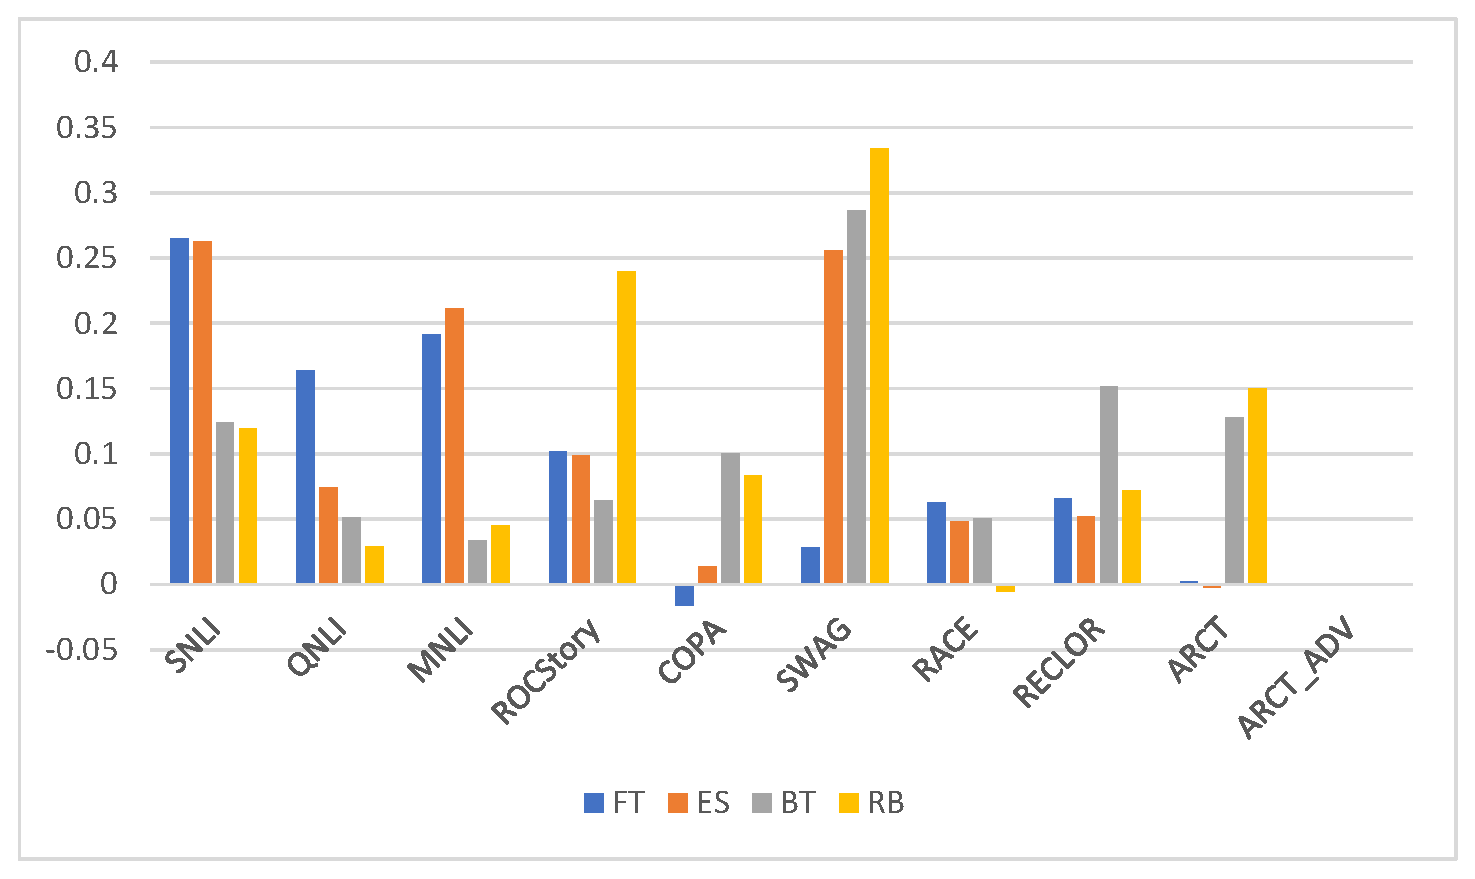
\includegraphics[width=\columnwidth]{picture/ending1.eps}
%\caption{Four models' hypothesis-only tests accuracies beyond vote by majority (hypo-only
%acc $-$ majority acc)}
%\label{fig:ending1}
%\end{figure}
%
%\begin{figure}[th]
%\centering
%\includegraphics[width=\columnwidth]{picture/ending2.eps}
%\caption{Four models' full test accuracies above hypothesis-only tests accuracies (full acc $-$
%hypo-only acc)}
%\label{fig:ending2}
%\end{figure}
%

\begin{table*}[th]
\centering
\scriptsize
\begin{tabular}{c|c|c|c|c|c|c|c|c|c|c|c} \hline
Dataset & Cue Type &Cue Value & Cueness & FT  & ES & BT & RB & FT  & ES & BT & RB\\ 
	&	&  & (LMI)  & ($\Delta$)& ($\Delta$)& ($\Delta$) & ($\Delta$)& (JSD)& (JSD)& (JSD)& (JSD) \\ \hline
\multirow{5}{*}{SNLI} 
&Tense&present&1.11&2.01&1.91&1.93&1.58&2.01e-02&1.91e-02&1.93e-02&1.58e-02\\
&Word&``.''&1.1&0.45&0.18&0.95&0.83&4.49e-03&1.82e-03&9.53e-03&8.30e-03\\
&Word&``a''&1.07&3.24&1.33&0.65&0.51&3.24e-02&1.33e-02&6.50e-03&5.14e-03\\
&Word&``the''&1.06&2.89&1.79&1.44&1.09&2.89e-02&1.79e-02&1.44e-02&1.09e-02\\
&Word&``is''&1.05&0.7&1.17&0.61&0.85&7.01e-03&1.17e-02&6.14e-03&8.46e-03\\
	   \hline 
\multirow{5}{*}{QNLI} 
&Word&``.''&1.08&8.57&11.84&6.78&4.46&8.57e-02&1.18e-01&6.78e-02&4.46e-02\\
&Word&``the''&1.07&1.43&2.2&0.67&0.06&1.43e-02&2.20e-02&6.67e-03&6.47e-04\\
&Tense&past&1.07&6.41&0.16&0.83&0.06&6.41e-02&1.58e-03&8.32e-03&5.57e-04\\
&Tense&present&1.07&1.02&5.85&2.87&2.4&1.02e-02&5.85e-02&2.87e-02&2.40e-02\\
&Word&``,''&1.06&1.83&2.54&0.18&0.74&1.83e-02&2.54e-02&1.76e-03&7.40e-03\\
	   \hline 
\multirow{5}{*}{MNLI} 
&Word&``.''&1.09&1.5&1.82&1.49&0.44&1.50e-02&1.82e-02&1.49e-02&4.44e-03\\
&Tense&present&1.08&1.27&1.25&0.4&0.17&1.27e-02&1.25e-02&3.98e-03&1.74e-03\\
&Word&``the''&1.05&2.43&1.92&0.58&0.04&2.43e-02&1.92e-02&5.76e-03&4.04e-04\\
&Tense&past&1.05&0.2&1.14&0.76&1.23&1.96e-03&1.14e-02&7.63e-03&1.23e-02\\
&Sentiment&sent\_any&1.05&1.8&1.67&1.07&1.39&1.80e-02&1.67e-02&1.07e-02&1.39e-02\\
	   \hline 
\multirow{5}{*}{ROCStory} 
&Tense&present&1.07&6.49&0.38&0.44&1.42&6.49e-02&3.76e-03&4.43e-03&1.42e-02\\
&Ner&PERSON&1.06&3.15&2.53&2.18&2.08&3.15e-02&2.53e-02&2.18e-02&2.08e-02\\
&Sentiment&positive&1.06&2.12&6.78&4.98&4.29&2.12e-02&6.78e-02&4.98e-02&4.29e-02\\
&Word&``the''&1.06&4.57&2.25&1.65&2.11&4.57e-02&2.25e-02&1.65e-02&2.11e-02\\
&Word&``to''&1.04&4.0&0.19&1.59&2.84&4.00e-02&1.88e-03&1.59e-02&2.84e-02\\
	   \hline 
\multirow{5}{*}{COPA} 
&Sentiment&sent\_any&1.06&0.29&4.42&0.46&4.93&2.88e-03&4.42e-02&4.60e-03&4.93e-02\\
&Sentiment&negative&1.05&3.78&1.19&2.86&3.21&3.78e-02&1.19e-02&2.86e-02&3.21e-02\\
&Word&``a''&1.03&4.38&2.07&2.78&0.53&4.38e-02&2.07e-02&2.78e-02&5.34e-03\\
&Word&``i''&1.03&0.73&4.77&7.08&1.7&7.29e-03&4.77e-02&7.08e-02&1.70e-02\\
&Word&``he''&1.03&0.69&2.43&12.5&3.42&6.90e-03&2.43e-02&1.25e-01&3.42e-02\\
	    \hline 
\multirow{5}{*}{RECLOR} 
&Word&``are''&1.03&1.44&1.05&0.35&1.54&1.44e-02&1.05e-02&3.48e-03&1.54e-02\\
&Word&``it''&1.03&1.03&0.24&5.15&1.61&1.03e-02&2.36e-03&5.15e-02&1.61e-02\\
&Word&``than''&1.02&0.32&2.28&1.31&0.84&3.20e-03&2.28e-02&1.31e-02&8.40e-03\\
&Word&``for''&1.02&2.81&0.02&1.13&1.08&2.81e-02&2.11e-04&1.13e-02&1.08e-02\\
&Word&``be''&1.02&2.39&1.04&0.76&0.84&2.39e-02&1.04e-02&7.62e-03&8.40e-03\\
	   \hline 
\multirow{5}{*}{ARCT} 
&Negation&negation&1.08&3.49&10.04&6.28&8.23&3.49e-02&1.00e-01&6.28e-02&8.23e-02\\
&Word&``the''&1.06&2.3&2.5&5.32&0.51&2.30e-02&2.50e-02&5.32e-02&5.15e-03\\
&Sentiment&positive&1.05&8.15&0.39&1.04&2.26&8.15e-02&3.91e-03&1.04e-02&2.26e-02\\
&Word&``not''&1.05&2.54&7.45&0.97&11.96&2.54e-02&7.45e-02&9.66e-03&1.20e-01\\
&Word&``to''&1.04&6.94&6.22&7.49&0.17&6.94e-02&6.22e-02&7.49e-02&1.74e-03\\
	   \hline
\multirow{5}{*}{ARCT2} 
&Negation&negation&1.06&0.29&2.05&0.06&1.45&2.90e-03&2.05e-02&5.54e-04&1.45e-02\\
&Word&``the''&1.05&0.29&1.09&1.39&0.0&2.90e-03&1.09e-02&1.39e-02&0.00e+00\\
&Sentiment&positive&1.05&2.71&0.85&0.52&0.0&2.71e-02&8.46e-03&5.17e-03&0.00e+00\\
&Word&``to''&1.04&1.14&2.44&0.04&1.06&1.14e-02&2.44e-02&3.92e-04&1.06e-02\\
&Tense&future&1.04&2.29&2.24&0.44&1.9&2.29e-02&2.24e-02&4.40e-03&1.90e-02\\
\hline
Model weakness & & & & 104.06 & 103.65 & 89.97 & 75.86 &0.3592&0.1993&0.1942&0.1854 \\
\hline 
\end{tabular}
\caption{Top 5 cues calculated by LMI for 8 datasets with their cueness scores and their corresponding accuracy test ($\Delta$) scores and distribution test (JSD) scores.}\label{tab:bias}
\end{table*}

\subsection{Cueness Metric Test}
%\subsection{Biases in Models}
We compute the MRR between the list of all candidate features ranked 
by cueness and the list of
top 20 features ranked by the accuracy test and distribution test scores. 
For a certain feature $w$ in candidate cues of models,  its reciprocal rank is $\frac{1}{rank_w}$ 
where $rank$ is the position of this feature in the list ranked by a cueness metric, like LMI.
Let $Q$ be a set of top 20 cues by accuracy or distribution test, the MRR is the mean of $Q$ reciprocal ranks:

\begin{equation}
\frac{1}{|Q|}\sum_{w \in Q}\frac{1}{rank_{w}}
\end{equation}
%\KZ{Give formula here of MRR?}
If the model does pick up the cue according to a cueness metric, 
then the MRR will be higher.
\figref{fig:cue_result} shows these MRR scores in 16 separate charts, 
one for each dataset and test. (a)-(h) is for accuracy test and (i)-(p) is for distribution test. 
From these experiments, it is clear that
LMI and Freq are better cueness metrics almost in every datasets and models except for ARCT2. 
Besides, LMI has a slight advantage over
frequency in SNLI, MNLI and ARCT. So we will use LMI as our choice of
cueness metric next.


\subsection{Cues in Datasets and Model Weakness}

Column 2 and 3 of \tabref{tab:bias} show the top 5 cues we have discovered
using LMI as the metric from all 8 datasets as well as their cueness scores.
We can see that present tense, negation, sentiment and gender oriented words such as
``he'' show up frequently in the list of top cues in these datasets. 
Person names turn out to be a useful cue in ROCStory which are made up of
short storys, and this makes good sense.
In line with previous reports, SNLI is the most biased datasets among the three
NLI datasets, the word ``a'' has been mentioned as a cue word in COPA~\cite{kavumbabalanced-copa}, and ARCT2, having been neutralized manually from ARCT, is less
biased than it's predecessor. For example, the LMI score for Negation on is a lower than 

%We further compute the normalized cueness per problem instance for these datasets
%by 
%\begin{equation}
%norm\_cueness (T) = \frac{1}{|p_i| \times |T|} \sum_{p_i \in T} \sum_{w \in p_i} cueness(w) 
%\end{equation}
%where $T$ is the training set, $p_i$ is a problem instance in $T$, and $w$ is a cue
%in $T$ with support of at least 100.

%\KZ{Results show that xxx is ...}
%ARCT2 is an adversarial dataset
%and is known to be well balanced on purpose. As a result, we only managed to find one cue
%which is OVERLAP and its cueness score is very low. This is not surprising, because
%OVERLAP is the only ``second-order'' feature in our list of linguistic features that
%is concerned with tokens in both the premise and hypothesis, and likely escaped from
%the data manipulation by the creator. 

%\begin{table}[th]
%\centering
%\scriptsize
%\begin{tabular}{|c|cc|cc|cc|} \hline
%Dataset & \multicolumn{2}{c|}{Freq} & \multicolumn{2}{c|}{CP} & \multicolumn{2}{c|}{LMI} \\ \hline
%\multirow{5}{*}{SNLI} 
%& ``sleeping'' & 13.95 & 30.3 &6.81 & 5.34& 4.87 \\                                                                    
%& ``no'' & 13.33 & 18.09 &3.32 & 2.05& 2.6 \\
%& ``because'' & 9.24 & 18.89 &4.88 & 5.61& 4.31 \\
%& ``friend'' & 8.82 & 22.96 &6.66 & 3.51& 3.05 \\
%& ``movie'' & 7.73 & 16.64 &0.06 & 9.47& -0.19 \\
%	   \hline 
%\multirow{5}{*}{QNLI} 
%& ``dioxide'' & 4.52 & 9.78 &-0.06 & 4.97& 10.56 \\                                                                    
%& ``denver'' & 4.26 & 13.59 &7.14 & 2.23& 3.11 \\
%& ``kilometre'' & 4.24 & 4.85 &6.43 & 4.67& 2.55 \\
%& ``mile'' & 3.95 & 7.16 &15.64 & -1.65& -6.65 \\
%& ``newcastle'' & 3.8 & 3.44 &12.0 & 0.89& -1.23 \\
%	   \hline 
%\multirow{5}{*}{MNLI} 
%& ``never'' & 10.4 & 29.15 &26.41 & 9.86& 10.6 \\                                                                      
%& ``no'' & 8.98 & 19.49 &20.17 & 1.2& 3.32 \\
%& ``nothing'' & 8.98 & 25.5 &26.84 & 5.11& 4.32 \\
%& ``any'' & 6.79 & 20.4 &19.39 & 7.76& 3.74 \\
%& ``anything'' & 5.73 & 18.43 &15.74 & 3.31& 1.14 \\
%	   
%	   \hline 
%\multirow{5}{*}{ROCStory} 
%& ``threw'' & 12.99 & 1.28 &4.69 & 10.88& 0.97 \\                                                                      
%& ``now'' & 8.68 & -10.01 &14.51 & 1.75& 5.69 \\
%& ``found'' & 8.16 & -2.31 &4.45 & 5.12& -3.13 \\
%& ``won'' & 7.71 & 2.43 &0.74 & 1.05& 5.51 \\
%& ``like'' & 7.3 & 4.77 &10.06 & 8.81& 1.67 \\
%	   \hline 
%\multirow{5}{*}{COPA} 
%& ``went'' & 3.61 & -10.83 &6.46 & 7.92& 1.04 \\                                                                       
%& ``got'' & 2.74 & 5.45 &-9.89 & -12.52& -10.3 \\
%& ``for'' & 2.14 & 10.11 &-1.89 & 9.05& 11.58 \\
%& ``with'' & 1.38 & -15.64 &-6.98 & 3.3& 13.82 \\
%& TYPO & 0.84 & -12.46 &-2.33 & 3.8& -8.22 \\
%	    \hline 
%\multirow{5}{*}{SWAG}
%& ``football'' & 7.38 & 6.13 &8.55 & 1.2& 1.55 \\
%& ``anxious'' & 6.65 & 7.55 &-4.67 & -6.66& -1.67 \\
%& ``concerned'' & 6.19 & 12.6 &4.58 & 8.27& -5.66 \\
%& ``skull'' & 5.73 & -2.77 &0.49 & 8.43& 3.49 \\
%& ``cop'' & 5.01 & 2.79 &5.3 & -0.92& -0.04 \\
%\hline 
%
%\multirow{5}{*}{RACE} 
%& ``above'' & 13.74 & 8.73 &-8.43 & -0.22& -1.92 \\                                                                    
%& ``b'' & 12.84 & 16.97 &-4.8 & 3.52& -3.45 \\
%& ``c'' & 11.83 & 15.69 &-6.94 & 8.6& -7.6 \\
%& ``probably'' & 6.77 & 9.91 &-0.06 & -3.8& 2.86 \\
%& ``may'' & 4.2 & 7.75 &-3.45 & -6.67& -1.8 \\
%	   
%	   \hline 
%\multirow{5}{*}{RECLOR} 
%& ``over'' & 2.07 & 1.76 &-2.94 & -1.35& -4.12 \\                                                                      
%& ``result'' & 1.97 & -3.29 &-2.69 & -1.78& -3.7 \\
%& ``explanation'' & 1.81 & -6.33 &-1.73 & -2.76& -7.24 \\
%& ``proportion'' & 1.68 & -5.64 &-4.69 & 2.37& -2.16 \\
%& ``produce'' & 1.4 & 4.54 &-2.98 & -14.36& -3.7 \\
%	   \hline 
%\multirow{5}{*}{ARCT} 
%& ``not'' & 3.74 & -2.54 &7.45 & -0.97& -11.96 \\                                                                      
%& NEGATION & 2.85 & 3.49 &10.04 & 6.28& -8.23 \\
%& ``n't'' & 2.52 & 10.3 &5.89 & 9.49& 4.84 \\
%& ``always'' & 2.25 & -4.66 &38.21 & -4.35& -8.26 \\
%& ``doe'' & 2.06 & -0.73 &-3.69 & -1.15& -7.22 \\
%	   \hline 
%ARCT\_adv& OVERLAP & 1.96e-10 & 1.65 &-0.25 & 2.73& 0.57 \\\hline
%\end{tabular}
%\caption{Top 5 cues and their cueness scores by three different metrics.}\label{tab:bias}
%\end{table}
%

%In most of the datasets, the top 5 cues discovered are word features,
%but besides OVERLAP, we do see NEGATION and TYPO showing up
%in the lists. In fact, SENTIMENT and NER features would have shown up
%if we expanded the list to top 10. It is also interesting to see several features previously
%reported to be biased by other works, such as ``not'' and NEGATION in
%ARCT, ``no'' in MNLI and SNLI, and ``like'' in ROCStory.  Especially in
%MNLI, all the five cues discovered are related to negatively toned words,
%suggesting significant human artifacts in this datasets.
% 
%In the results, we also identify that some of the word cues are indicative of
%certain syntactic/semantic/sentiment patterns in the questions. For example, ``because'' in SNLI
%indicates a causal-effect structure; ``like'' in ROCStory indicates positive sentiment;
%``probably'' and ``may'' in RACE indicate uncertainty, etc. 
%

%The only exception is SWAG, which didn't emerge as a very
%weak dataset in the experiment here, but was found very biased in
%the hypothesis-only test. The reason is SWAG is the biggest dataset
%among the ten and we discovered more cues in it than
%the other 9 combined. Therefore, the top 5 cues are insufficient
%to represent the full scale of its weakness, which is showed by
%the hypothesis test as it gives the full picture.

%\begin{figure}[th]
%\centering
%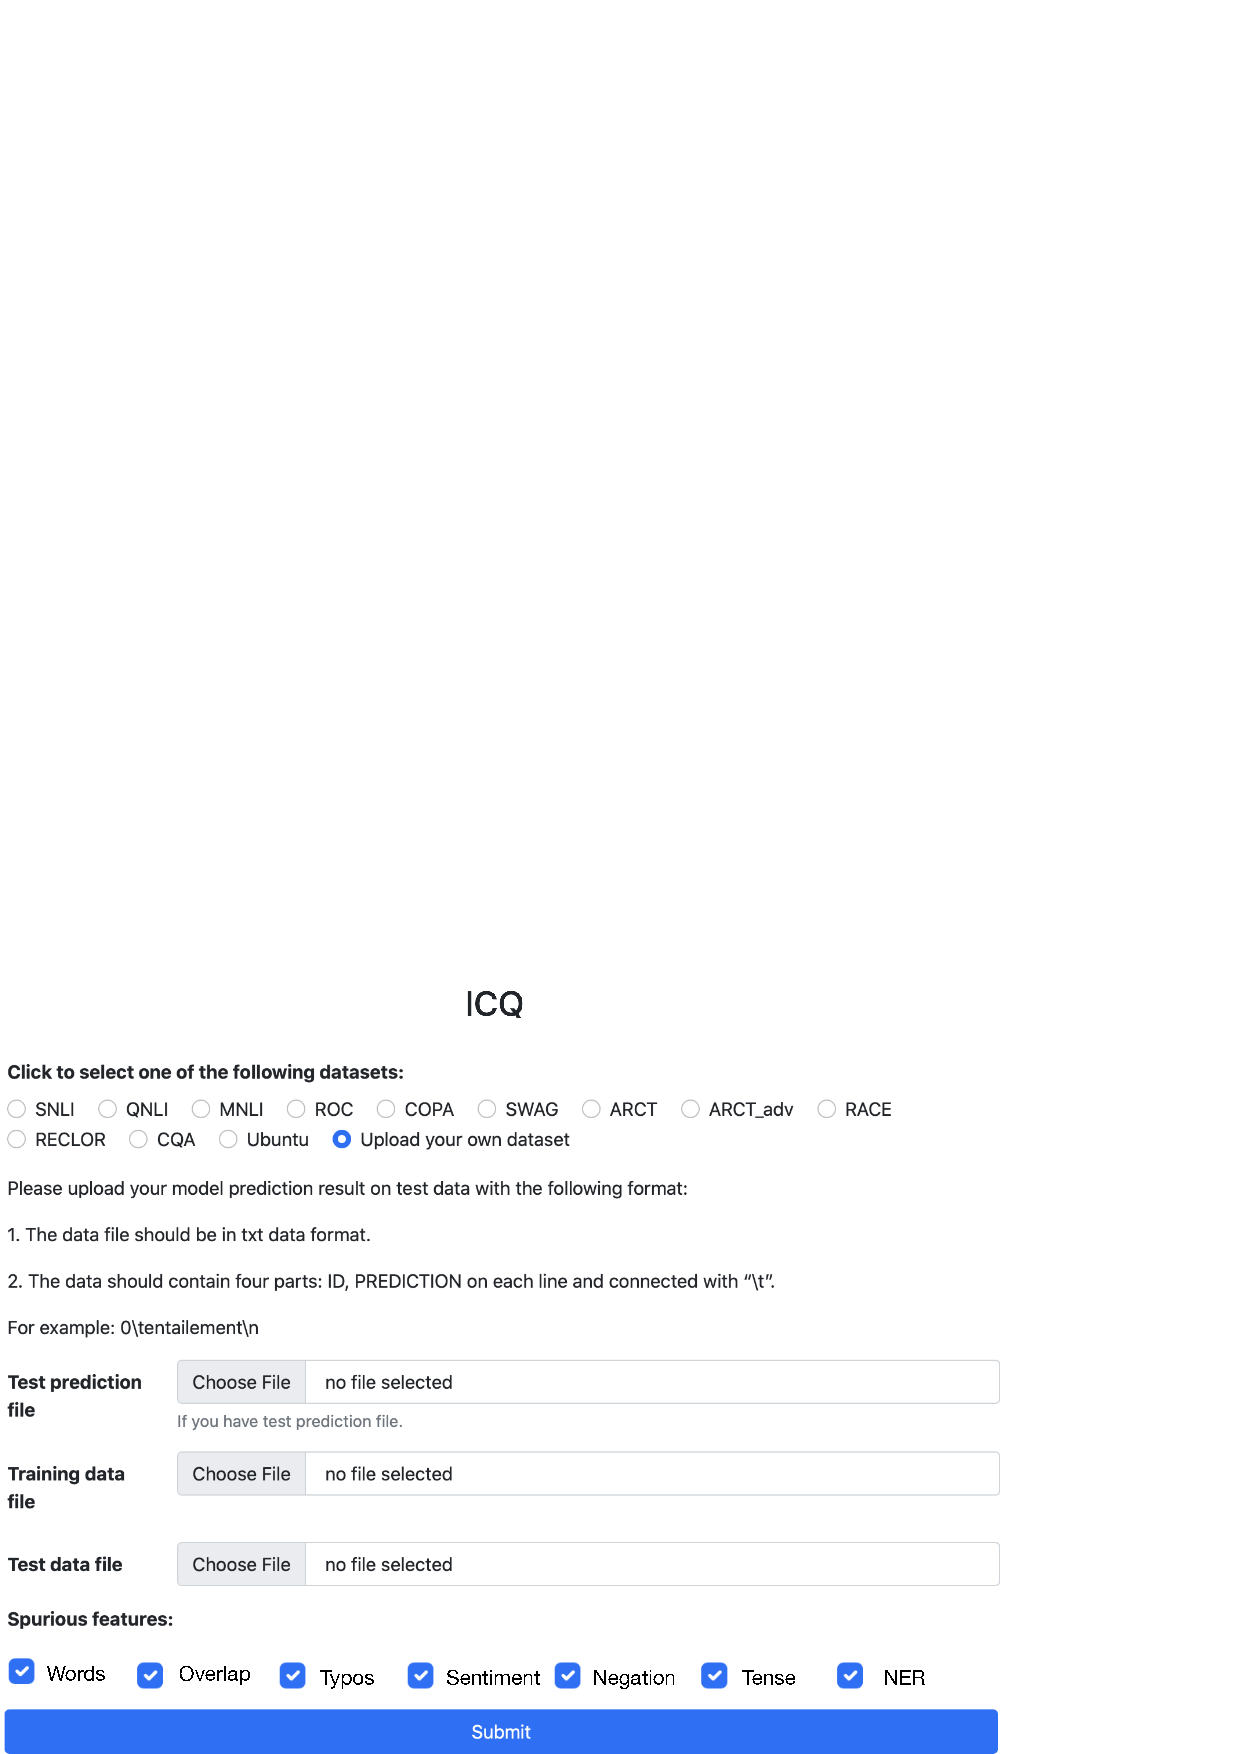
\includegraphics[width=1.0\columnwidth]{picture/dataset.jpg}
%\caption{Dataset Evaluation Panel}
%\label{fig:dataset}
%\end{figure}

Next we turn to the model's weakness against these cues.
When we sum up the $\Delta$ scores and JSD scores for both tests
in the 8 columns to the right of \tabref{tab:bias}. 
We called the sum ``model weakness'' in an informal way.
We can see that by accuracy test and distribution test,
the overall model weaknesses are:  
RoBERTA $<$ BERT $<$ ESIM $<$ FastText. 
This again is consistent with 
the community's common perception of these popular models.
The model-dependent scores also show relatively good consistence with
the ranking of model independent cueness scores (LMI), that is, the
bigger $\Delta$ and JSD scores appear on the top for each model and dataset.

%For example, it seems that FastText tends to pick up more individual word cues
%than semantic cues, but more complex models such as BERT
%and RoBERTA appear to be more sensitive to structural features such as NEGATION
%and SENTIMENT, which are actually classes of words. 
%This can be well explained by the way FastText is designed to
%model words more than syntactic or semantic structures.
%
%The fact that FastText is strongly negatively correlated with TYPO is
%also interesting. We speculate that FastText might have been
%trained with a more orthodoxical vocabulary and thus less
%tolerant to typos in text. 

\cut{%%%%%%%%%%%%%%%%%%%%%%%%%
\subsubsection{Distribution Test}

\begin{figure*}[th]
\centering
\begin{subfigure}[b]{0.3\textwidth}
\centering
\includegraphics[width=\columnwidth]{picture/no_mnli.eps}
\caption{Cue ``no'' in MNLI}
\label{fig:cue_no}
\end{subfigure}
\hfill
\begin{subfigure}[b]{0.3\textwidth}
\centering
\includegraphics[width=\columnwidth]{picture/above_arct.eps}
\caption{Cue ``above'' in ARCT}
\label{fig:cue_above}
\end{subfigure}
\hfill
\begin{subfigure}[b]{0.3\textwidth}
\centering
\includegraphics[width=\columnwidth]{picture/threw_roc.eps}
\caption{Cue ``threw'' in ROCStory}
\label{fig:cue_threw}
\end{subfigure}
\caption{Three test examples for distribution comparison with 4 different models}
\label{fig:cue_result}
\end{figure*}


%With previous experiment, we can find that many 
%models are positively correlated with various of features, 
%like ``no'' in MNLI.
%However, it is still not enough to confirm that the models greatly 
%rely on this feature only to make the decision. 
%The inflence of other feature or coincidence can also cause 
%a high accuracy. 
We further invesigate the models using the
``distribution test''. 
%It is 
%easily to understand if a model fully influenced by this feature, 
%this model will be more inclined to choose the side 
%with more data in the training. We can observing the imbalance 
%of the distribution to judge if a model really interested with 
%these shallow features. 
We show three insteresting findings in \figref{fig:cue_result}. 
We observe that all models on cue ``no'' in MNLI 
achieve positive $\Delta$ in \tabref{tab:bias}, and fastText in particular. 
%It means this cue have a great chance to inflence models. 
Consistent with the ``Accuracy test'', we find the predicting label distribution 
skewness is amplified in \figref{fig:cue_no} for fastText and ESIM -  
with ``no'' in sight, they prefer to predict ``Contradiction'' even more
than the ground truth in training data.
On the contrary, BERT and RoBERTA are only moderate in following
the training data. 

If cue ``no'' is very good at tricking the models,
cue ``above'' is not as successful. 
\figref{fig:cue_above} shows that 
%the distribution test for models on cue ``above'' in ARCT 
the distribution of predicting result for ESIM in ARCT 
is completely opposite to the training data. 
This explains while $\Delta=-8.43$ in \tabref{tab:bias} and
demonstrates that models may not take advantage of the cue even though it is
right there in the data.
Similarly, the ``flatness'' in BERT and RoBERTA 
can also explain their low $\Delta$ values in \tabref{tab:bias}. 

The example of cue ``threw'' presents an outlier for BERT,
because the distribution test result is inconsistent between the accuracy test: 
The accuracy deviation is very high for BERT, but its prediction distribution is
flat. We haven't seen a lot of such contradictory cases so far. 
But when it happens, as it is here, we give BERT the benefit of the doubt 
that it might not have exploited the cue ``threw''. 

}%%%%%%%%%%%%%%%%%% end of cut %%%%%%%%
%\begin{figure}[th]
%\centering
%\includegraphics[width=1.0\columnwidth]{picture/model_result.jpg}
%\caption{Examples of Evaluating Models}
%\label{fig:model_result}
%\end{figure}
%We proceed to demonstrate the effectiveness of our framework in two aspects:
%First, 
%we use our method to detect cues and measure the amount of information leak
%in 12 datasets from 6 different tasks, as shown in~\tabref{tab:datasets_exp}. 
%Second, we evaluate the true reasoning power of a number of popular NLP
%models on original test sets that are split into 
%easy and hard part. 

%\begin{table*}[th]
%\centering:
%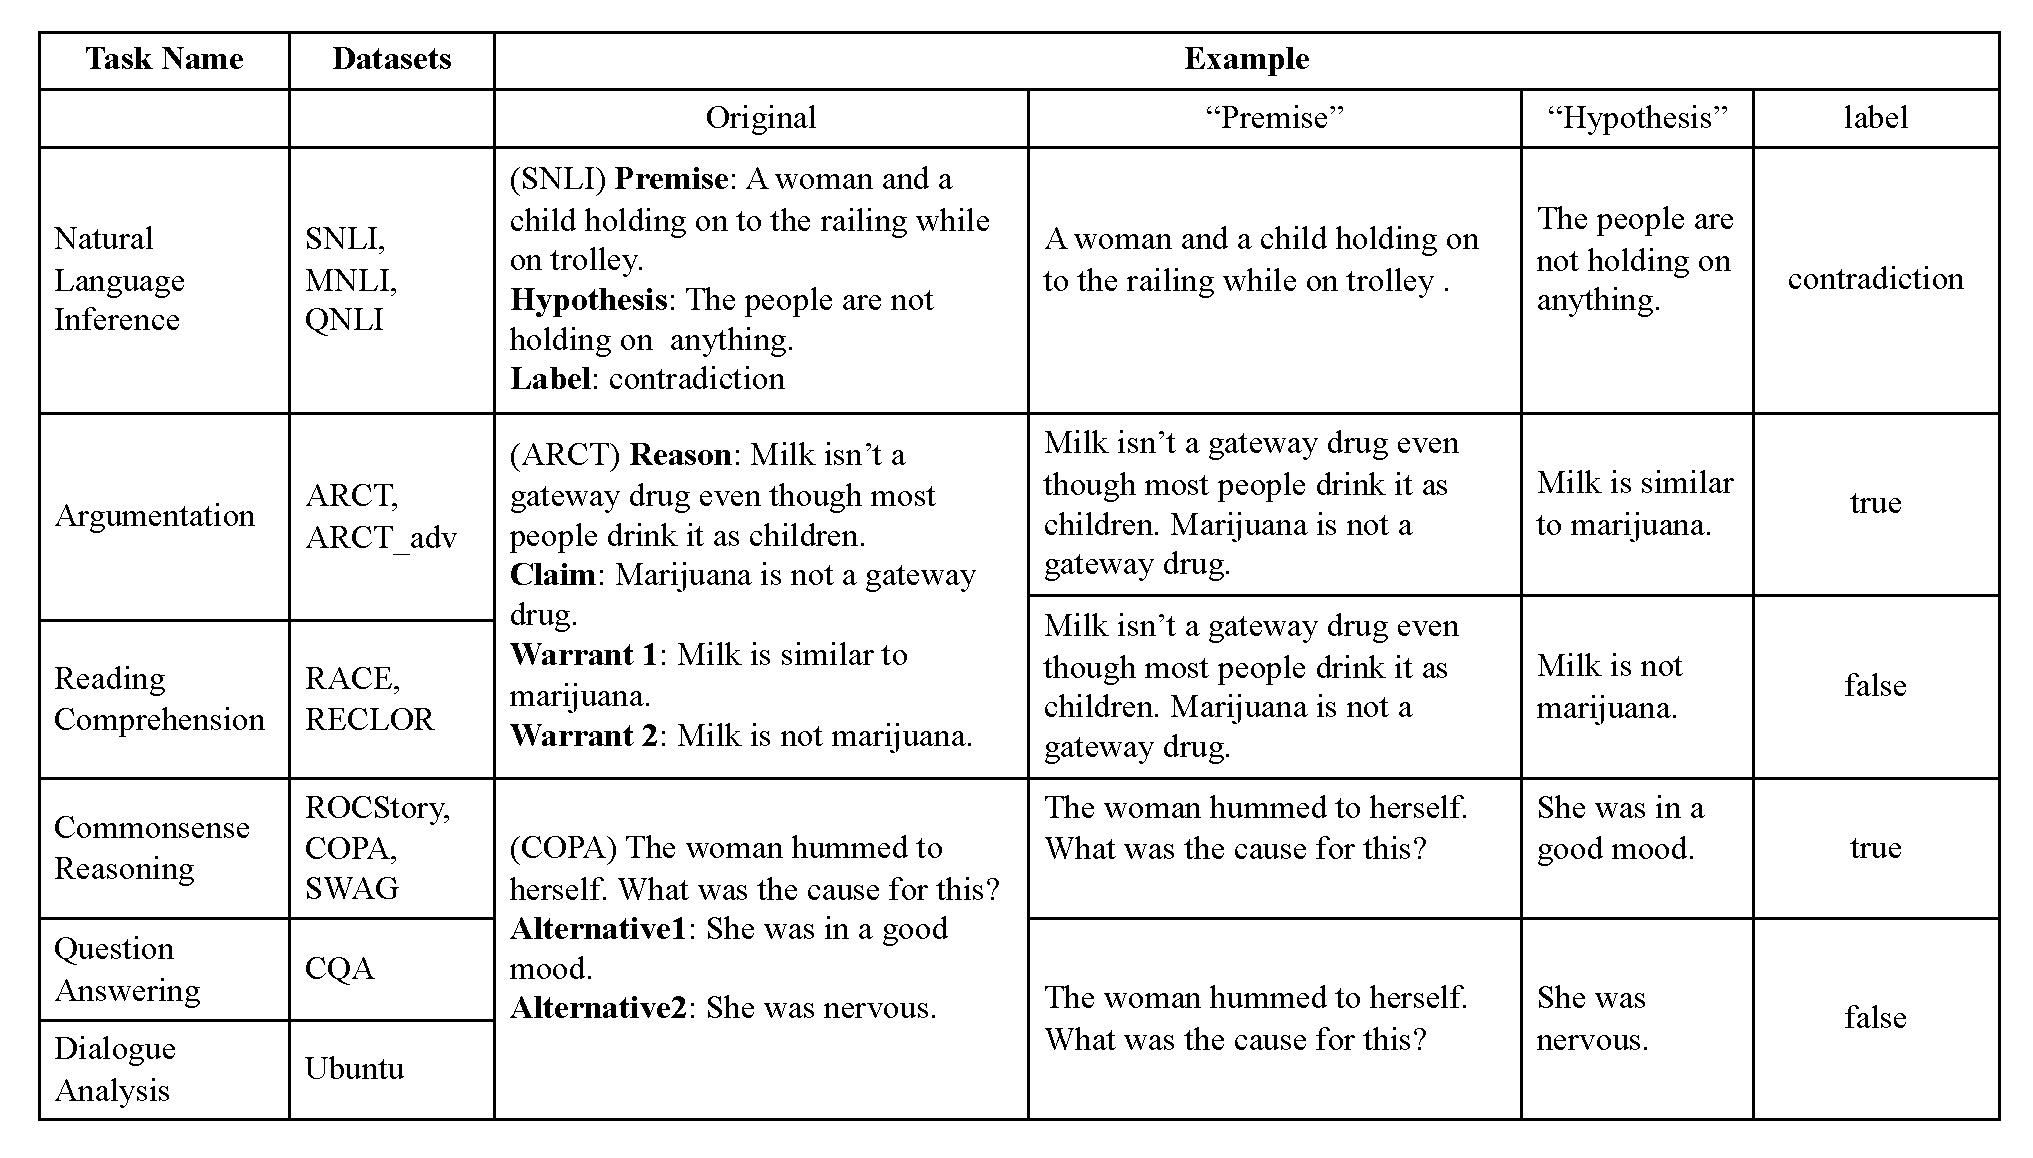
\includegraphics[width=2\columnwidth]{picture/datasets_exp.eps}
%\caption{Data examples and normalized version.}
%\label{tab:datasets_exp}
%\end{table*}
%

